\chapter{Simulations and observables}\label{ch: parameters}
In this chapter we will present some basic information on the implementation of the previously discussed algorithm and state the utilized parameters of the conducted simulations. Furthermore we need to discuss how to take the continuum limit of the observables of interest.
%
%
%
% - - - - - - -   implementation and sim param   - - - - - - - -
%
%
%
\section{Implementation and the continuum limit}
The executables for the Monte Carlo simulation are built from an implementation in the \names{Fortran 95} standard and are compiled with an $\text{Intel}^{\circledR}$ \texttt{ifort} compiler\footnote{From the $\text{Intel}^{\circledR}$ Parallel Studio XE 2015.}. For the lattice we deploy several sizes for the spatial extent $L=8,10,12,16,24,32$, whereas the temporal extent is always twice of the spatial one $T=2L$ for an improved accuracy of the bosonic correlators. Thus we have a world volume of $V_{2}=2a^{2}L^{2}$. In the continuum model there are two "bare" parameters that determine its behaviour, the dimensionless coupling $g=\sqrt{\lambda}/4\pi$ and the mass scale $m$. To take the continuum limit it is necessary to set a line of constant physics when $a \to 0$ which is said to be the squared physical mass of the field excitations rescaled with the world volume
%
%
\begin{equation}
V_{2}m_{x}^{2} = \text{const}.
\label{eq: line_of_c_phys1}
\end{equation}
%
%
From a dimensional regularization scheme it is possible to find the corrections to the masses of the bosonic fields $x,x^{*}$ which read \cite{Giombi:2010bj}
%
%
\begin{equation}
m_{x}^{2}(g) = \frac{m^{2}}{2}\left(1 - \frac{1}{8g} + \mathcal{O}(g^{-2}) \right).
\label{eq: m_x}
\end{equation}
%
%
Together with (\ref{eq: line_of_c_phys1}) and for a fixed value of $g$ this leads to 
%
%
\begin{equation}
\frac{V_{2}m^{2}}{2} = (LM)^{2} = \text{const},
\label{eq: line_of_c_phys2}
\end{equation}
%
%
where $M=ma$ is the dimensionless lattice mass scale. The equality (\ref{eq: line_of_c_phys2}) relies on the hypothesis that $g$ is not (infinitely) renormalized\footnote{This argument can be substantiated by our perturbative knowledge of the scaling function. One could define $f(g)/4 = g + \text{const.} + \mathcal{O}(g^{-1})$ as a renormalized coupling. Since it is linear in $g$ up to first order and does not depend on a renormalization scale, the $\beta$-function is zero and $g$ needs no renormalization.}. Further the validity of (\ref{eq: m_x}) in the discretized model needs to be verified in order the physical masses undergo only a finite renormalization. This claim is supported by studying $x,x^{*}$ correlators where indeed no presence of $(1/a)$ divergences in the $m_{x}^{2}/m^{2}$ ratios can be found. Also for the large $g$ region they reach their expected continuum value of $1/2$. Having this in mind and also the result of the perturbative 1-loop free energy (\ref{eq: 1_loop}), we assume no further presence of a scale in the discretized model other than the lattice spacing $a$. Therefore any expectation value of an observable $\langle F_{\rm LAT}\rangle$ is a function of the "bare" input parameters $g,L$ and $M$
%
%
\begin{equation}
\langle F_{\rm LAT}\rangle = \langle F_{\rm LAT}(g,L,M)\rangle = \langle F(g) \rangle + \mathcal{O}(L^{-1}) + \mathcal{O}\left( e^{-LM}\right).
\end{equation}
%
%
For fixed $g$ one chooses a fixed $LM$, large enough to keep finite volume effects $\mathcal{O}\left( e^{-LM}\right)$ small. For each finite value $L$ there will be a difference of $\langle F_{\rm LAT}\rangle$ and its continuum equivalent by means of lattice artefacts $\mathcal{O}(L^{-1})$. The continuum limit $\langle F(g) \rangle$ is obtained via an extrapolation to infinite $L$.
%
%
%
%
%
%  - - - - - - - -  simulation parameters   - - - - - - - - - - - 
%
%
%
%
\section{Simulation parameters}
As mentioned we employ different lattice sizes varying between $L=8$ and $L=32$. In the HMC simulation the MD equations of motion are evaluated along a fictitious MC time $\tau$. For one trajectory we utilize a MC time of $\tau = 0.5$ with by default 100 integrator steps and therefore $\epsilon=\delta\tau = 0.005$. For the fractional powers of the fermion matrix we use a rational approximation (\ref{eq: rat_approx}) of degree $P=15$ with the two sets of parameters stated in \autoref{tab: rat_app_coef}. We checked for a subset of the configurations that its accuracy is always better than $10^{-3}$ for $\xi^{\dagger}\big(\mathcal{O}_{\rm F}^{\dagger}\mathcal{O}_{\rm F}\big)^{-\frac{1}{4}}\xi$.
%
%
%\begin{table}[h]
\begin{longtable}{ccll}
\toprule
$\rho$ &$i$ &  \hspace{2cm}$\alpha_{i}$ &  \hspace{2cm}$\beta_{i}$ \\ 
\midrule
  & 0 & $\hspace{10pt} 3.2148873149863206$ & \hspace{2cm}- \\ 
  & 1 & $-2.2977600408751347\cdot 10^{-9}$ & $5.5367335615411457\cdot 10^{-8}$ \\ 
  & 2 & $-1.6898103706901084\cdot 10^{-8}$ & $4.6910257304582898\cdot 10^{-7}$ \\ 
  & 3 & $-1.1099658368596436\cdot 10^{-7}$ & $2.6768223190551614\cdot 10^{-6}$ \\ 
  & 4 & $-7.2162146587729939\cdot 10^{-7}$ & $1.4319657256375662\cdot 10^{-5}$ \\ 
  & 5 & $-4.6841070484595924\cdot 10^{-6}$ & $7.5694473187855338\cdot 10^{-5}$ \\ 
  & 6 & $-3.0396303865820389\cdot 10^{-5}$ & $3.9922490005559548\cdot 10^{-4}$ \\ 
1/8  & 7 & $-1.9723870959636086\cdot 10^{-4}$ & $2.1046795395127538\cdot 10^{-3}$ \\ 
  & 8 & $-1.2798599250624023\cdot 10^{-3}$ & $1.1094832053548640\cdot 10^{-2}$ \\ 
  & 9 & $-8.3051856063983548\cdot 10^{-3}$ & $5.8486687698920667\cdot 10^{-2}$ \\ 
  & 10 & $-5.3904877281192094\cdot 10^{-2}$ & $3.0834388405073770\cdot 10^{-1}$ \\ 
  & 11 & $-3.5026088217184553\cdot 10^{-1}$ & $1.6264534005778293$ \\ 
  & 12 & $-2.2893521967679966$ & $8.6030459456576764$ \\ 
  & 13 & $-1.5436668340425719\cdot 10 $& $4.6179583183155444\cdot 10$ \\ 
  & 14 & $-1.2297861076048798\cdot 10^{2}$ & $2.6854965277696181\cdot 10^{2}$ \\ 
  & 15 & $-2.6252652966414048\cdot 10^{3} $& $2.6004158696112045\cdot 10^{3} $\\ 
%\bottomrule
%\end{tabular} 
%\caption{First set of coefficients used for the rational approximation (\ref{eq: rat_approx}) sufficient for the exponent $\rho = 1/8$. \label{tab: rat_app_coef1}}
%\end{table}
%\vspace{0.5cm}
%\begin{table}[ht!]
%\begin{tabular}{ccll}
%\toprule
%$\rho$ &$i$ &  \hspace{2cm}$\alpha_{i}$ &  \hspace{2cm}$\beta_{i}$ \\ 
\midrule
  & 0 & $9.5797060554725838\cdot 10^{-2}$ & \hspace{2cm}- \\ 
  & 1 & $1.7701746700099842\cdot 10^{-6}$ & $3.1085594175442315\cdot 10^{-8}$ \\ 
  & 2 & $5.8705983656937455\cdot 10^{-6}$ & $3.2994455960441383\cdot 10^{-7}$ \\ 
  & 3 & $1.9961158693570120\cdot 10^{-5}$ & $1.9424842756552213\cdot 10^{-6}$ \\ 
  & 4 & $6.9125367600088173\cdot 10^{-5}$ & $1.0453359626231250\cdot 10^{-5}$ \\ 
  & 5 & $2.4032965323696816\cdot 10^{-4}$ & $5.5337819905761986\cdot 10^{-5}$ \\ 
  & 6 & $8.3620125835371663\cdot 10^{-4}$ & $2.9204178440857227\cdot 10^{-4}$ \\ 
-1/4  & 7 & $2.9099006745502945\cdot 10^{-3}$  & $1.5403300046437174\cdot 10^{-3}$ \\ 
  & 8 & $1.0126504714418652\cdot 10^{-2}$ & $8.1233558140562465\cdot 10^{-3}$ \\ 
  & 9 & $3.5241454044660878\cdot 10^{-2}$ & $4.2840454273820550\cdot 10^{-2}$ \\ 
  & 10 & $1.2266034741624667\cdot 10^{-1}$ & $2.2594500626442715\cdot 10^{-1}$ \\ 
  & 11 & $4.2721681852328125\cdot 10^{-1}$ & $1.1921171782283737$ \\ 
  & 12 & 1.4932820692676758 & 6.3026182343759860 \\ 
  & 13 & 5.3188766358452595 & $3.3683411978650057\cdot 10$ \\ 
  & 14 & $2.0944763089672641\cdot 10^{1}$ & $1.9083658214156412\cdot 10^{2}$ \\ 
  & 15 & $1.4525770103354523\cdot 10^{2}$ & $1.5386784635765257\cdot 10^{3}$ \\ 
\bottomrule
\caption{Two sets of coefficients used for the rational approximation (\ref{eq: rat_approx}) sufficient for the exponents $\rho = 1/8$ and $\rho=-1/4$, respectively. \label{tab: rat_app_coef}}
\end{longtable} 
%\end{table}
%
%
In \autoref{tab: runs_param} we list the parameters of the simulations presented in this thesis. For each set of parameters we collected a certain amount of data points. Their total number would cover a trajectory of the length of the corresponding MDU value stated in the table. In most cases data has been collected along independent trajectories, launched from different start configurations which are referred to as replica. These can be used to improve statistics. We also determined auto-correlation times of the main observables, the correlator $\langle x^{*}x\rangle$ and the action $\langle S_{\rm cusp} \rangle$ (which will be subject of the next section), and included their effect in the error analysis \cite{Wolff:2003sm}.
%
%
%
\begin{longtable}{cccccccc}
\toprule
$g$ & $T\times L$ & $LM$ & $r$ & $\tau_{\rm int}^{S}\,(Q)$ & $\tau_{\rm int}^{m_x}\,(Q)$ & R & MDU \\
\midrule
 10 & $16 \times   8$ &  4 & 1 & 0.6 \; (0.6) & 1.8 \; (0.5) & 4 & 2826 \\
    & $20 \times  10$ &  4 & 1 & 0.7 \; (0.5) & 2.0 \; (0.4) & 3 & 2652 \\
    & $24 \times  12$ &  4 & 1 & 0.7 \; (0.6) & 0.0 \; (0.8) & 4 & 2666 \\
    & $32 \times  16$ &  4 & 1 & 0.7 \; (0.4) & 3.0 \; (0.5) & 4 & 3802 \\
    & $48 \times  24$ &  4 & 1 & 0.7 \; (0.3) & 6.2 \; (0.2) & 3 & 2702 \\
    & $64 \times  32$ &  4 & 1 & 0.6 \; (0.7) & 6.3 \; (1.0) & 4 & 1073 \\
\midrule
 15 & $16 \times   8$ &  4 & 1 & 2.1 \; (0.6) & 1.6 \; (0.9) & 5 & 4553 \\
    & $20 \times  10$ &  4 & 1 & 2.0 \; (0.5) & 1.5 \; (0.2) & 5 & 4553 \\
    & $24 \times  12$ &  4 & 1 & 2.1 \; (0.1) & 1.5 \; (0.0) & 5 & 4553 \\
    & $32 \times  16$ &  4 & 1 & 2.5 \; (0.7) & 2.2 \; (0.4) & 5 & 4553 \\
    & $48 \times  24$ &  4 & 1 & 2.0 \; (-) & 2.5 \; (-) & 1 & 925 \\
\midrule
 20 & $16 \times   8$ &  4 & 1 & 35.8 \; (0.4) & 4.0 \; (0.4) & 21 & 19961 \\
    & $20 \times  10$ &  4 & 1 & 41.6 \; (0.4) & 1.4 \; (0.5) & 21 & 19961 \\
    & $24 \times  12$ &  4 & 1 & 31.2 \; (0.1) & 1.4 \; (0.0) & 21 & 19961 \\
    & $32 \times  16$ &  4 & 1 & 42.2 \; (0.3) & 1.9 \; (0.6) & 21 & 19961 \\
    & $48 \times  24$ &  4 & 1 & 23.3 \; (0.6) & 3.3 \; (0.7) & 4 & 3602 \\
    & $64 \times  32$ &  4 & 1 & 55.7 \; (0.3) & 4.5 \; (0.9) & 4 & 1338 \\
\midrule
 25 & $16 \times   8$ &  4 & 1 & 2.3 \; (0.6) & 1.5 \; (0.0) & 19 & 18060 \\
    & $20 \times  10$ &  4 & 1 & 2.5 \; (0.2) & 3.8 \; (0.1) & 20 & 19010 \\
    & $24 \times  12$ &  4 & 1 & 2.5 \; (0.1) & 1.9 \; (0.3) & 20 & 19010 \\
    & $32 \times  16$ &  4 & 1 & 2.6 \; (0.6) & 2.5 \; (0.0) & 20 & 19010 \\
    & $48 \times  24$ &  4 & 1 & 2.4 \; (0.3) & 2.4 \; (0.4) & 5 & 4553 \\
    & $64 \times  32$ &  4 & 1 & 2.5 \; (0.7) & 2.7 \; (0.4) & 2 & 560 \\
\midrule
 30 & $16 \times   8$ &  4 & 1 & 1.0 \; (0.2) & 1.6 \; (0.9) & 17 & 16159 \\
    & $20 \times  10$ &  4 & 1 & 1.0 \; (0.2) & 2.4 \; (0.9) & 20 & 18810 \\
    & $24 \times  12$ &  4 & 1 & 1.0 \; (1.0) & 2.0 \; (0.1) & 20 & 18810 \\
    & $32 \times  16$ &  4 & 1 & 1.1 \; (0.7) & 1.6 \; (0.7) & 20 & 18810 \\
    & $48 \times  24$ &  4 & 1 & 1.0 \; (0.7) & 2.3 \; (0.0) & 20 & 18010 \\
    & $64 \times  32$ &  4 & 1 & 1.1 \; (0.1) & 4.8 \; (0.0) & 5 & 2050 \\
\midrule
 40 & $16 \times   8$ &  4 & 1 & 0.5 \; (1.0) & 1.4 \; (0.1) & 18 & 17109 \\
    & $20 \times  10$ &  4 & 1 & 0.7 \; (0.6) & 1.5 \; (0.0) & 20 & 19010 \\
    & $24 \times  12$ &  4 & 1 & 0.6 \; (1.0) & 2.8 \; (0.2) & 20 & 19010 \\
    & $32 \times  16$ &  4 & 1 & 0.6 \; (0.1) & 1.4 \; (0.5) & 20 & 19010 \\
    & $48 \times  24$ &  4 & 1 & 0.7 \; (0.8) & 1.9 \; (0.1) & 5 & 5449 \\
\midrule
 50 & $16 \times   8$ &  4 & 1 & 0.7 \; (0.5) & 1.4 \; (0.0) & 20 & 19010 \\
    & $20 \times  10$ &  4 & 1 & 0.7 \; (0.9) & 1.4 \; (0.9) & 20 & 19010 \\
    & $24 \times  12$ &  4 & 1 & 0.8 \; (1.0) & 1.4 \; (0.2) & 20 & 19010 \\
    & $32 \times  16$ &  4 & 1 & 0.8 \; (0.5) & 2.1 \; (1.0) & 20 & 18852 \\
    & $48 \times  24$ &  4 & 1 & 0.8 \; (0.0) & 1.8 \; (0.6) & 5 & 4451 \\
\midrule
100 & $16 \times   8$ &  4 & 1 & 1.1 \; (0.4) & 3.9 \; (0.1) & 2 & 1701 \\
    & $20 \times  10$ &  4 & 1 & 1.0 \; (0.9) & 4.2 \; (0.4) & 2 & 1701 \\
    & $24 \times  12$ &  4 & 1 & 1.2 \; (0.7) & 1.9 \; (0.6) & 2 & 1701 \\
    & $32 \times  16$ &  4 & 1 & 1.1 \; (0.6) & 1.6 \; (0.5) & 2 & 1701 \\
    & $48 \times  24$ &  4 & 1 & 1.1 \; (-) & 1.7 \; (-) & 1 & 751 \\
\midrule
  5 & $16 \times   8$ &  4 & 1 & 0.5 \; (-) & 1.5 \; (-) & 1 & 3591 \\
    & $24 \times  12$ &  4 & 1 & 0.4 \; (0.1) & 3.1 \; (0.0) & 4 & 3752 \\
    & $32 \times  16$ &  4 & 1 & 0.6 \; (0.0) & 4.4 \; (0.1) & 5 & 4703 \\
\midrule
 30 & $16 \times   8$ &  4 & 1 & 1.0 \; (0.9) & 1.6 \; (0.4) & 4 & 9802 \\
    & $24 \times  12$ &  4 & 1 & 1.0 \; (0.6) & 1.6 \; (0.3) & 4 & 9802 \\
    & $32 \times  16$ &  4 & 1 & 1.0 \; (0.7) & 1.5 \; (1.0) & 2 & 4901 \\
\midrule
 40 & $16 \times   8$ &  4 & 1 & 0.6 \; (0.1) & 1.3 \; (0.2) & 4 & 9802 \\
    & $24 \times  12$ &  4 & 1 & 0.6 \; (0.9) & 2.9 \; (0.4) & 4 & 9802 \\
    & $32 \times  16$ &  4 & 1 & 0.7 \; (0.5) & 1.7 \; (0.1) & 2 & 4901 \\
\midrule
 50 & $16 \times   8$ &  4 & 1 & 0.8 \; (0.7) & 1.5 \; (0.4) & 4 & 9802 \\
    & $24 \times  12$ &  4 & 1 & 0.7 \; (0.0) & 1.5 \; (0.9) & 4 & 9802 \\
    & $32 \times  16$ &  4 & 1 & 0.8 \; (0.9) & 2.1 \; (0.9) & 2 & 4901 \\
\midrule
 60 & $16 \times   8$ &  4 & 1 & 1.1 \; (0.9) & 2.1 \; (0.8) & 2 & 19901 \\
    & $24 \times  12$ &  4 & 1 & 1.1 \; (-) & 1.5 \; (-) & 1 & 9951 \\
    & $32 \times  16$ &  4 & 1 & 0.9 \; (0.2) & 2.9 \; (1.0) & 2 & 2171 \\
    & $48 \times  24$ &  4 & 1 & 0.9 \; (-) & 2.2 \; (-) & 1 & 751 \\
\midrule
 70 & $16 \times   8$ &  4 & 1 & 3.0 \; (0.0) & 3.8 \; (0.7) & 2 & 19901 \\
    & $24 \times  12$ &  4 & 1 & 3.5 \; (0.9) & 1.3 \; (0.9) & 2 & 19901 \\
    & $32 \times  16$ &  4 & 1 & 3.1 \; (0.1) & 1.9 \; (0.9) & 2 & 5049 \\
    & $48 \times  24$ &  4 & 1 & 3.5 \; (-) & 1.8 \; (-) & 1 & 751 \\
\midrule
100 & $20 \times  10$ &  6 & 1 & 1.2 \; (0.4) & 11.3 \; (0.1) & 3 & 2652 \\
    & $24 \times  12$ &  6 & 1 & 1.0 \; (0.3) & 4.3 \; (0.1) & 5 & 4553 \\
    & $32 \times  16$ &  6 & 1 & 1.2 \; (0.9) & 2.0 \; (0.2) & 4 & 3802 \\
    & $48 \times  24$ &  6 & 1 & 1.4 \; (0.9) & 1.5 \; (0.0) & 5 & 1541 \\
\midrule
 70 & $24 \times  12$ &  6 & 1 & 2.7 \; (0.7) & 1.7 \; (0.1) & 5 & 4553 \\
    & $32 \times  16$ &  6 & 1 & 3.0 \; (0.6) & 2.6 \; (0.8) & 4 & 3802 \\
    & $40 \times  20$ &  6 & 1 & 4.4 \; (0.5) & 1.8 \; (0.4) & 4 & 4002 \\
    & $48 \times  24$ &  6 & 1 & 3.0 \; (0.3) & 1.6 \; (0.5) & 5 & 1431 \\
\midrule
 50 & $24 \times  12$ &  6 & 1 & 0.6 \; (0.6) & 1.6 \; (0.5) & 5 & 4553 \\
    & $32 \times  16$ &  6 & 1 & 0.7 \; (0.9) & 1.8 \; (0.0) & 5 & 4553 \\
    & $40 \times  20$ &  6 & 1 & 0.7 \; (0.3) & 1.7 \; (0.6) & 4 & 4002 \\
    & $48 \times  24$ &  6 & 1 & 0.6 \; (0.0) & 3.8 \; (0.0) & 5 & 1333 \\
\midrule
 30 & $20 \times  10$ &  6 & 1 & 1.0 \; (0.3) & 2.3 \; (0.2) & 5 & 4553 \\
    & $24 \times  12$ &  6 & 1 & 1.0 \; (0.2) & 2.1 \; (1.0) & 5 & 4553 \\
    & $32 \times  16$ &  6 & 1 & 1.1 \; (0.1) & 1.6 \; (0.6) & 5 & 4553 \\
    & $40 \times  20$ &  6 & 1 & 1.0 \; (0.8) & 1.7 \; (0.3) & 4 & 4002 \\
    & $48 \times  24$ &  6 & 1 & 1.0 \; (0.9) & 1.7 \; (0.0) & 5 & 1216 \\
\midrule
 25 & $20 \times  10$ &  6 & 1 & 2.5 \; (0.4) & 3.2 \; (0.0) & 5 & 4553 \\
    & $24 \times  12$ &  6 & 1 & 2.5 \; (0.8) & 1.7 \; (0.0) & 5 & 4553 \\
    & $32 \times  16$ &  6 & 1 & 2.6 \; (0.4) & 2.3 \; (0.4) & 5 & 4553 \\
    & $40 \times  20$ &  6 & 1 & 2.5 \; (0.7) & 1.5 \; (0.6) & 4 & 4002 \\
\midrule
 20 & $20 \times  10$ &  6 & 1 & 30.8 \; (0.3) & 1.6 \; (0.6) & 5 & 4553 \\
    & $24 \times  12$ &  6 & 1 & 41.5 \; (0.2) & 1.4 \; (0.7) & 5 & 4553 \\
    & $32 \times  16$ &  6 & 1 & 47.9 \; (0.3) & 1.6 \; (0.7) & 5 & 4553 \\
    & $40 \times  20$ &  6 & 1 & 91.1 \; (1.0) & 1.7 \; (0.0) & 4 & 4002 \\
\midrule
 15 & $20 \times  10$ &  6 & 1 & 2.2 \; (0.1) & 2.0 \; (0.1) & 5 & 4553 \\
    & $24 \times  12$ &  6 & 1 & 2.3 \; (0.3) & 1.6 \; (0.7) & 5 & 4553 \\
    & $32 \times  16$ &  6 & 1 & 2.0 \; (0.9) & 1.6 \; (0.0) & 5 & 4553 \\
\midrule
 10 & $20 \times  10$ &  6 & 1 & 0.6 \; (0.4) & 2.3 \; (0.5) & 5 & 4553 \\
    & $24 \times  12$ &  6 & 1 & 0.6 \; (0.1) & 1.8 \; (0.9) & 5 & 4553 \\
    & $32 \times  16$ &  6 & 1 & 0.7 \; (0.3) & 2.1 \; (0.0) & 5 & 4553 \\
\midrule
 25 & $16 \times   8$ &  4 & 0 & 2.2 \; (0.8) & 1.5 \; (0.6) & 5 & 4553 \\
    & $20 \times  10$ &  4 & 0 & 2.0 \; (0.9) & 2.1 \; (0.3) & 5 & 4553 \\
    & $24 \times  12$ &  4 & 0 & 2.2 \; (0.0) & 1.7 \; (0.4) & 5 & 4553 \\
    & $32 \times  16$ &  4 & 0 & 1.9 \; (0.1) & 2.6 \; (0.8) & 5 & 4553 \\
\midrule
 30 & $16 \times   8$ &  4 & 0 & 0.9 \; (0.4) & 1.4 \; (0.1) & 5 & 4553 \\
    & $20 \times  10$ &  4 & 0 & 0.8 \; (0.0) & 1.5 \; (0.2) & 5 & 4553 \\
    & $24 \times  12$ &  4 & 0 & 0.9 \; (0.7) & 1.7 \; (0.1) & 5 & 4553 \\
    & $32 \times  16$ &  4 & 0 & 1.1 \; (0.9) & 2.2 \; (0.3) & 5 & 4553 \\
\midrule
 50 & $16 \times   8$ &  4 & 0 & 0.6 \; (0.0) & 1.6 \; (0.2) & 5 & 4553 \\
    & $20 \times  10$ &  4 & 0 & 0.7 \; (0.2) & 1.5 \; (0.0) & 5 & 4553 \\
    & $24 \times  12$ &  4 & 0 & 0.7 \; (0.4) & 1.5 \; (0.4) & 5 & 4553 \\
    & $32 \times  16$ &  4 & 0 & 0.7 \; (0.0) & 1.6 \; (0.3) & 5 & 4553 \\
\midrule
 70 & $16 \times   8$ &  4 & 0 & 2.7 \; (0.6) & 3.1 \; (0.3) & 5 & 4553 \\
    & $20 \times  10$ &  4 & 0 & 2.7 \; (0.4) & 1.4 \; (0.6) & 5 & 4553 \\
    & $24 \times  12$ &  4 & 0 & 3.3 \; (0.7) & 1.4 \; (0.0) & 8 & 6404 \\
    & $32 \times  16$ &  4 & 0 & 3.4 \; (0.3) & 2.2 \; (0.1) & 5 & 4553 \\
\midrule
 80 & $16 \times   8$ &  4 & 0 & 24.9 \; (0.2) & 7.2 \; (0.0) & 5 & 4553 \\
    & $20 \times  10$ &  4 & 0 & 32.4 \; (0.2) & 1.7 \; (0.2) & 5 & 4553 \\
    & $24 \times  12$ &  4 & 0 & 35.8 \; (0.6) & 1.4 \; (0.5) & 8 & 6404 \\
    & $32 \times  16$ &  4 & 0 & 13.9 \; (0.1) & 1.5 \; (0.5) & 5 & 4553 \\
\midrule
100 & $16 \times   8$ &  4 & 0 & 1.0 \; (0.3) & 2.5 \; (0.5) & 5 & 4553 \\
    & $20 \times  10$ &  4 & 0 & 1.1 \; (0.5) & 3.4 \; (1.0) & 5 & 4553 \\
    & $24 \times  12$ &  4 & 0 & 1.0 \; (0.6) & 1.5 \; (0.0) & 5 & 4553 \\
    & $32 \times  16$ &  4 & 0 & 1.2 \; (0.2) & 1.5 \; (0.0) & 5 & 4553 \\
\bottomrule\\
\caption{Parameters of the simulation: the coupling $g$, the temporal $(T)$ and spacial $(L)$ extent of the lattice, the line of constant physics fixed by $LM$ and the presence of a \names{Wilson} term, toggled by $r$ to be included during the simulation (1) or not (0). The size of the statistics after thermalization is given in the last column in terms of molecular dynamic units (MDU) which equals an HMC trajectory of length one. The number of replica collected for each set of parameters is stated in the column named R. The auto-correlation times $\tau$ of our main observables $m_{x}$ and $S$ are also given in MDU together with the Q-value of the replica in parenthesis. \label{tab: runs_param}}
\end{longtable}

%
%
%
The meaning of the Q-value, given in the table, is defined in \cite{Wolff:2003sm}. It reveals information about the quality of an observable with respect to their replica. One derives the mean value for each replicum and analyses the distribution of these means in comparison to the total mean of all replica. The Q-value is of cause more meaningful if there is a high number of replica. \\
%
\begin{figure}
\centering
% This file was created by matlab2tikz.
%
%The latest updates can be retrieved from
%  http://www.mathworks.com/matlabcentral/fileexchange/22022-matlab2tikz-matlab2tikz
%where you can also make suggestions and rate matlab2tikz.
%
\definecolor{mycolor1}{rgb}{0.00000,0.44700,0.74100}%
\definecolor{mycolor2}{rgb}{0.85000,0.32500,0.09800}%
\definecolor{mycolor3}{rgb}{0.92900,0.69400,0.12500}%
%
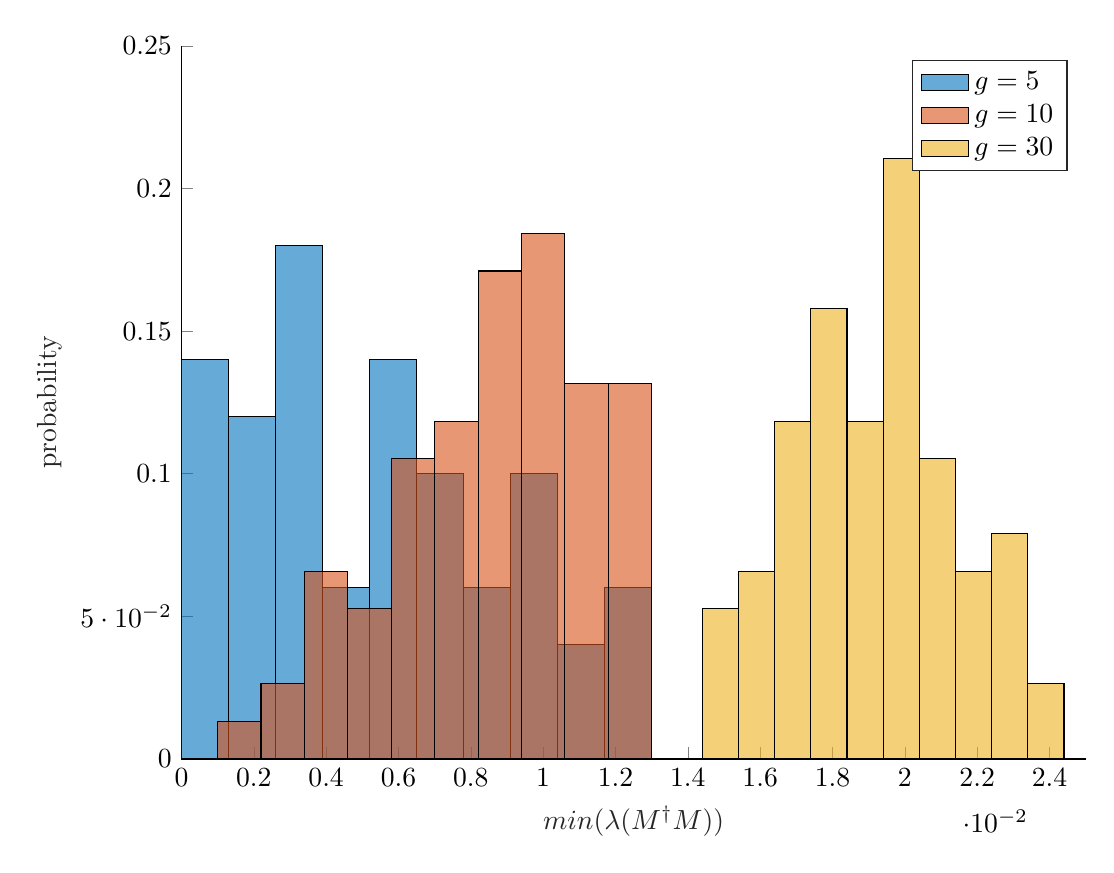
\begin{tikzpicture}

\begin{axis}[%
width=4.521in,
height=3.566in,
at={(0.758in,0.481in)},
scale only axis,
xmin=0,
xmax=0.025,
xlabel style={font=\color{white!15!black}},
xlabel={$min(\lambda(M^\dagger M))$},
ymin=0,
ymax=0.25,
ylabel style={font=\color{white!15!black}},
ylabel={probability},
axis background/.style={fill=white},
axis x line*=bottom,
axis y line*=left,
legend style={legend cell align=left, align=left, draw=white!15!black}
]
\addplot[ybar interval, fill=mycolor1, fill opacity=0.6, draw=black, area legend] table[row sep=crcr] {%
x	y\\
0	0.14\\
0.0013	0.12\\
0.0026	0.18\\
0.0039	0.06\\
0.0052	0.14\\
0.0065	0.1\\
0.0078	0.06\\
0.0091	0.1\\
0.0104	0.04\\
0.0117	0.06\\
0.013	0.06\\
};
\addlegendentry{$g = 5$}

\addplot[ybar interval, fill=mycolor2, fill opacity=0.6, draw=black, area legend] table[row sep=crcr] {%
x	y\\
0.001	0.0131578947368421\\
0.0022	0.0263157894736842\\
0.0034	0.0657894736842105\\
0.0046	0.0526315789473684\\
0.0058	0.105263157894737\\
0.007	0.118421052631579\\
0.0082	0.171052631578947\\
0.0094	0.184210526315789\\
0.0106	0.131578947368421\\
0.0118	0.131578947368421\\
0.013	0.131578947368421\\
};
\addlegendentry{$g = 10$}

\addplot[ybar interval, fill=mycolor3, fill opacity=0.6, draw=black, area legend] table[row sep=crcr] {%
x	y\\
0.0144	0.0526315789473684\\
0.0154	0.0657894736842105\\
0.0164	0.118421052631579\\
0.0174	0.157894736842105\\
0.0184	0.118421052631579\\
0.0194	0.210526315789474\\
0.0204	0.105263157894737\\
0.0214	0.0657894736842105\\
0.0224	0.0789473684210526\\
0.0234	0.0263157894736842\\
0.0244	0.0263157894736842\\
};
\addlegendentry{$g = 30$}

\end{axis}
\end{tikzpicture}%
\hspace{0.2cm}
% This file was created by matlab2tikz.
%
%The latest updates can be retrieved from
%  http://www.mathworks.com/matlabcentral/fileexchange/22022-matlab2tikz-matlab2tikz
%where you can also make suggestions and rate matlab2tikz.
%
\definecolor{mycolor1}{rgb}{0.00000,0.44700,0.74100}%
\definecolor{mycolor2}{rgb}{0.85000,0.32500,0.09800}%
\definecolor{mycolor3}{rgb}{0.92900,0.69400,0.12500}%
%
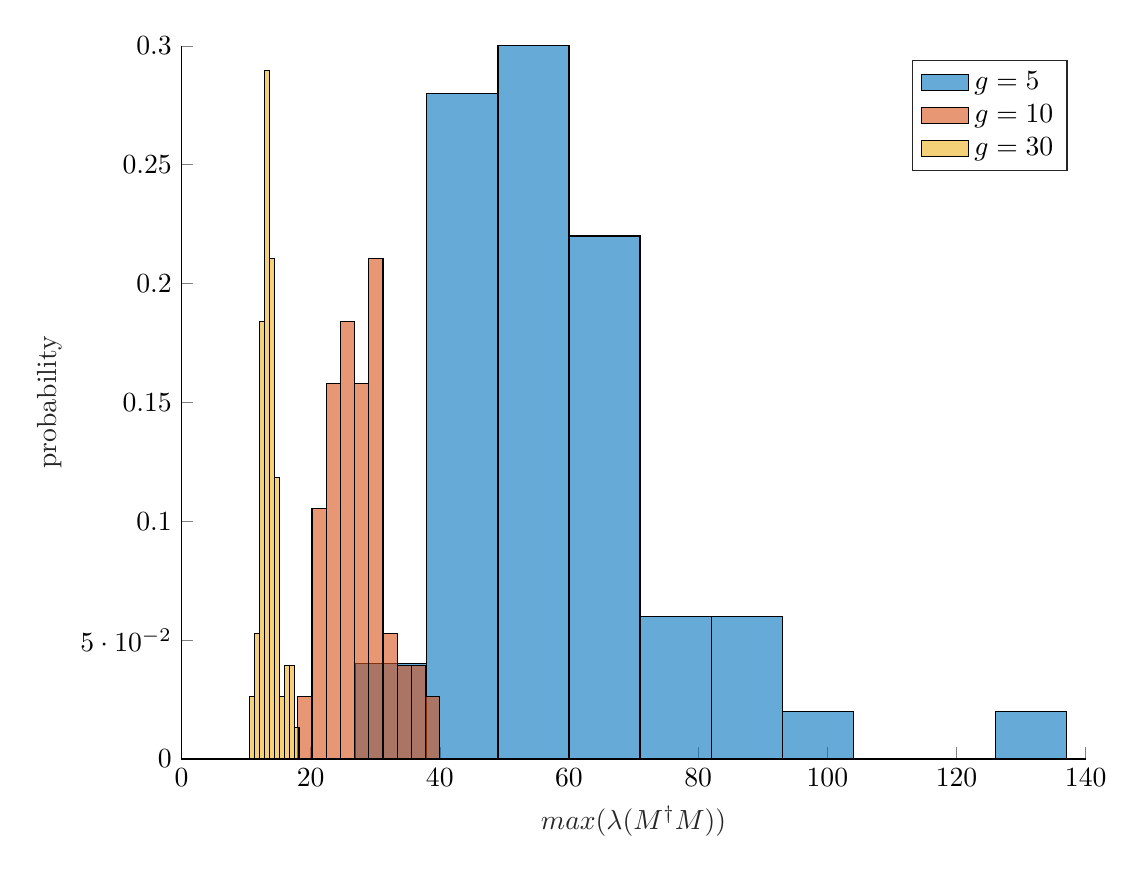
\begin{tikzpicture}

\begin{axis}[%
width=4.521in,
height=3.566in,
at={(0.758in,0.481in)},
scale only axis,
xmin=0,
xmax=140,
xlabel style={font=\color{white!15!black}},
xlabel={$max(\lambda(M^\dagger M))$},
ymin=0,
ymax=0.3,
ylabel style={font=\color{white!15!black}},
ylabel={probability},
axis background/.style={fill=white},
axis x line*=bottom,
axis y line*=left,
legend style={legend cell align=left, align=left, draw=white!15!black}
]
\addplot[ybar interval, fill=mycolor1, fill opacity=0.6, draw=black, area legend] table[row sep=crcr] {%
x	y\\
27	0.04\\
38	0.28\\
49	0.3\\
60	0.22\\
71	0.06\\
82	0.06\\
93	0.02\\
104	0\\
115	0\\
126	0.02\\
137	0.02\\
};
\addlegendentry{$g = 5$}

\addplot[ybar interval, fill=mycolor2, fill opacity=0.6, draw=black, area legend] table[row sep=crcr] {%
x	y\\
18	0.0263157894736842\\
20.2	0.105263157894737\\
22.4	0.157894736842105\\
24.6	0.184210526315789\\
26.8	0.157894736842105\\
29	0.210526315789474\\
31.2	0.0526315789473684\\
33.4	0.0394736842105263\\
35.6	0.0394736842105263\\
37.8	0.0263157894736842\\
40	0.0263157894736842\\
};
\addlegendentry{$g = 10$}

\addplot[ybar interval, fill=mycolor3, fill opacity=0.6, draw=black, area legend] table[row sep=crcr] {%
x	y\\
10.5	0.0263157894736842\\
11.27	0.0526315789473684\\
12.04	0.184210526315789\\
12.81	0.289473684210526\\
13.58	0.210526315789474\\
14.35	0.118421052631579\\
15.12	0.0263157894736842\\
15.89	0.0394736842105263\\
16.66	0.0394736842105263\\
17.43	0.0131578947368421\\
18.2	0.0131578947368421\\
};
\addlegendentry{$g = 30$}

\end{axis}
\end{tikzpicture}%
\caption{Histogram plot of the eigenvalue spectrum of one replicum with 400 field configurations for $L=12$ and $g=5,10,30$. For high values of $g$ the smallest eigenvalues are clearly separated from zero which ensures the stability of the simulation. With decreasing $g$ the smallest eigenvalues come arbitrarily close to zero whereas the largest eigenvalues increase at the same time which leads to high condition numbers of the fermionic operator and threatens the stability of the simulation. \label{fig: ev_dist}}
\end{figure}
%

Additional simulations have been conducted for fixed $LM=6$ to check for the influence of finite volume effects and with $r=0$ which means without the presence of a \names{Wilson} term to check its influence on the observables.\\
We can observe that for lower $g$ values the simulations become more involved. For too small values of $g$ the conjugate gradient method to solve (\ref{eq: mscg}) does not converge. This is due to the eigenvalue spectrum of the fermion matrix $\hat{\mathcal{O}}_{\rm F}$ shown in \autoref{fig: ev_dist}. For small $g$ the condition number of $\hat{\mathcal{O}}_{\rm F}$ (which is basically the ratio of the largest and smallest eigenvalue) becomes very bad. The smallest eigenvalues are so close to zero that they might leave the regime of accuracy of the rational approximation (\ref{eq: rat_approx}) and are within the range of errors of the conjugate gradient solver which could cause a phase transition of the \names{Pfaffian}. During our simulation with $LM=4$ and a present \names{Wilson} term this behaviour occurred for the first time for $g=5$ . We tried to cure this peculiarity with help of a reweighting procedure which was introduced first in \cite{Ferrenberg:1988yz} (see also \cite{Luscher:2008tw,Finkenrath:2013soa}). Therefore we add a twisted mass term to the fermionic matrix to obtain
%
%
\begin{align}
\tilde{\mathcal{O}}_{\rm F} &= \hat{\mathcal{O}}_{\rm F} + i\mu \Gamma_{5},  &
\tilde{\mathcal{O}}_{\rm F} \tilde{\mathcal{O}}_{\rm F}^{\dagger} &= \hat{\mathcal{O}}_{\rm F}\hat{\mathcal{O}}_{\rm F}^{\dagger} + \mu^{2}\mathds{1},
\end{align}
%
%
where $\mu$ is the reweighting mass parameter. The term $\mu^{2}\mathds{1}$ will shift the eigenvalues of $\tilde{\mathcal{O}}_{\rm F} \tilde{\mathcal{O}}_{\rm F}^{\dagger}$ apart from zero and ensures the stability of the simulation. Hereby the crucial term in measuring an observable is the \names{Pfaffian} which is included in the probability distribution in the RHMC. We want to estimate observables generated from a distribution without an additional mass term by actually doing simulations with a twisted mass. While assuming the \names{Pfaffian} to be positive we can write
%
%
\begin{equation}
\begin{alignedat}{2}
\pf\big(\hat{\mathcal{O}}_{\rm F}\big) &= \left(\frac{\det \big(\hat{\mathcal{O}}_{\rm F} \hat{\mathcal{O}}_{\rm F}^{\dagger} \big)}{\det \big(\tilde{\mathcal{O}}_{\rm F} \tilde{\mathcal{O}}_{\rm F}^{\dagger} \big)}\right)^{\frac{1}{4}} \pf\big(\tilde{\mathcal{O}}_{\rm F}\big)\\
%
&\equiv W \;\pf\left(\tilde{\mathcal{O}}_{\rm F}\right).
\end{alignedat}
\label{eq: rew_factor}
\end{equation}
%
%
For a small reweighting mass $\mu$ we can thus compute an estimate of the observable vev without the twisted mass $\langle O \rangle_{0}$ via
%
%
\begin{equation}
\langle O \rangle_{0} = \frac{\langle O W \rangle_{\mu}}{\langle W \rangle_{\mu}} .
\end{equation}
%
%
The vev $\langle O \rangle_{\mu}$ represents the value obtained from a RHMC simulation with twisted mass term and $W$ is the reweighting factor defined in (\ref{eq: rew_factor}). It can be expressed in terms of $\;\widetilde{\!W}=W^{4}$ which can be rewritten to
%
%
\begin{equation}
\widetilde{\!W} = \frac{\det \left(\hat{\mathcal{O}}_{\rm F}\hat{\mathcal{O}}_{\rm F}^{\dagger}\right)}{\det\left(\hat{\mathcal{O}}_{\rm F}\hat{\mathcal{O}}_{\rm F}^{\dagger}+ \mu^{2}\right)} = \frac{1}{\det\left( \mathds{1}+\frac{\mu^{2}}{\hat{\mathcal{O}}_{\rm F}\hat{\mathcal{O}}_{\rm F}^{\dagger}}\right)} \equiv \frac{1}{\det M}.
\end{equation}
%
%
In a separate MC integration we estimate $\;\widetilde{\!W}$ by using
%
%
\begin{equation}
\frac{1}{\det M} = \int \mathcal{D}\xi \; e^{-\xi^{\dagger}M\xi} = \int \mathcal{D}\xi\; \left(\frac{e^{-\xi^{\dagger}M\xi}}{\rho(\xi)}\right) \rho(\xi),
\end{equation}
%
%
where the complex fields $\xi$ are distributed according to $\rho(\xi)$ so that by (\ref{eq: vev_rho}) we can write
%
%
\begin{equation}
\frac{1}{\det M} = \left\langle \frac{e^{-\xi^{\dagger}M\xi}}{\rho(\xi)}\right\rangle_{\rho}.
\end{equation}
%
%
With a \names{Gaussian} distribution $\rho(\xi)=\exp(-\xi^{\dagger}\xi)$ we find the stochastic estimation
%
%
\begin{equation}
\begin{alignedat}{2}
\widetilde{\!W} &= \left\langle \exp \left[ -\xi^{\dagger}\left(\frac{\mu^{2}}{\hat{\mathcal{O}}_{\rm F}\hat{\mathcal{O}}_{\rm F}^{\dagger}}\right)\xi\right]\right\rangle_{\rho} \\
&= \frac{1}{N_{\xi}} \sum\limits_{k=1}^{N_{\xi}} \exp \left[ -\xi_{k}^{\dagger}\left(\frac{\mu^{2}}{\hat{\mathcal{O}}_{\rm F}\hat{\mathcal{O}}_{\rm F}^{\dagger}}\right)\xi_{k}\right] + \mathcal{O}\left(\frac{1}{\sqrt{N_{\xi}}}\right). 
\end{alignedat}
\end{equation}
%
%
The reweighting procedure is of cause also limited in its application and is only valid for small shifts $\mu$. We therefore choose $\mu$ as small a possible, but large enough to ensure the stability of the simulation. Reweighting has only been applied for the collection of data with $g=5$. A plot of the reweighting factors for a collection of field configurations is given in \autoref{fig: rew_factor}.
%
%
\begin{figure}
\centering
% This file was created by matlab2tikz.
%
%The latest updates can be retrieved from
%  http://www.mathworks.com/matlabcentral/fileexchange/22022-matlab2tikz-matlab2tikz
%where you can also make suggestions and rate matlab2tikz.
%
\definecolor{mycolor1}{rgb}{0.00000,0.44700,0.74100}%
%
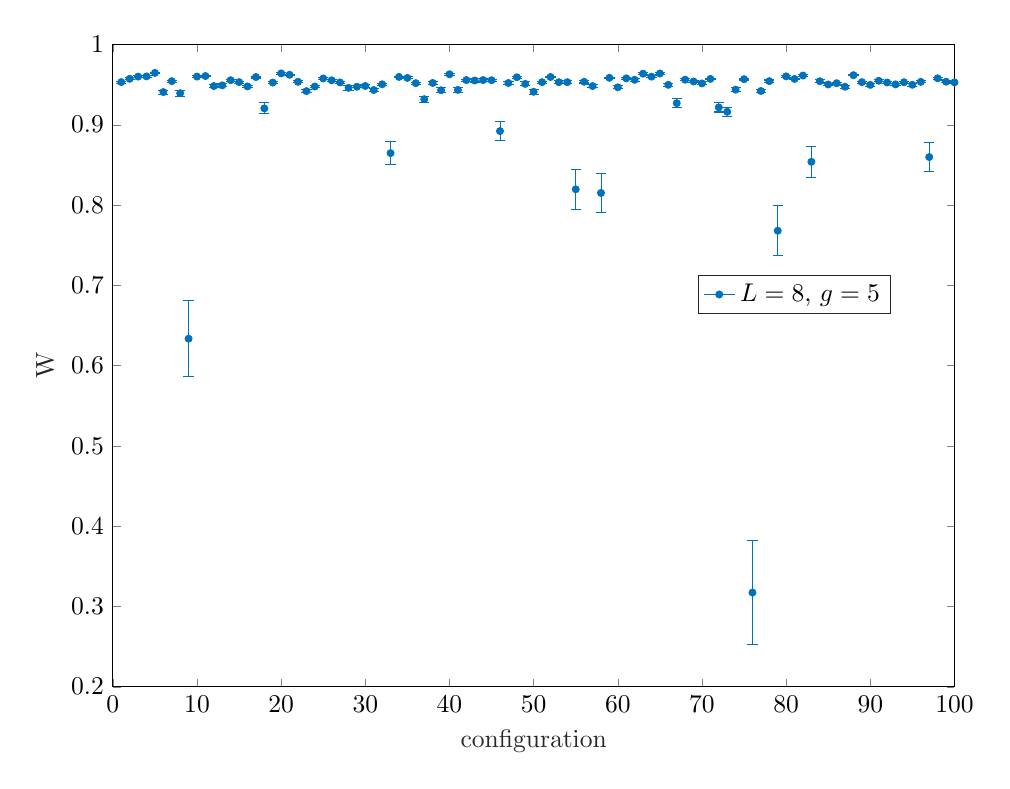
\begin{tikzpicture}[thick,scale=0.65, every node/.style={scale=1.42}]

\begin{axis}[%
width=6.474in,
height=4.941in,
at={(1.086in,0.667in)},
scale only axis,
xmin=0,
xmax=100,
xlabel style={font=\color{white!15!black}},
xlabel={configuration},
ymin=0.2,
ymax=1,
ylabel style={font=\color{white!15!black}},
ylabel={W},
axis background/.style={fill=white},
legend style={at={(0.695,0.580)}, anchor=south west, legend cell align=left, align=left, draw=white!15!black}
]
\addplot [color=mycolor1, draw=none, mark=*, mark options={solid, mycolor1}]
 plot [error bars/.cd, y dir = both, y explicit]
 table[row sep=crcr, y error plus index=2, y error minus index=3]{%
1	0.953030237078629	0.00133252750175868	0.00133252750175868\\
2	0.957150503958378	0.00119541958365667	0.00119541958365667\\
3	0.959889343761428	0.000938639147507316	0.000938639147507316\\
4	0.960154724973424	0.000980984469972055	0.000980984469972055\\
5	0.964550865872029	0.000885901666303172	0.000885901666303172\\
6	0.940630342232228	0.00250014555798991	0.00250014555798991\\
7	0.95425368547006	0.00134627394156228	0.00134627394156228\\
8	0.939178886966104	0.00364762466007334	0.00364762466007334\\
9	0.633457123731367	0.0472812228023222	0.0472812228023222\\
10	0.959909327569502	0.00103165385055101	0.00103165385055101\\
11	0.960636529655091	0.000993794898290946	0.000993794898290946\\
12	0.948113096374446	0.00164624057217347	0.00164624057217347\\
13	0.948987707828379	0.00176526783317368	0.00176526783317368\\
14	0.955407054926832	0.00102583085103299	0.00102583085103299\\
15	0.95301757863849	0.00132418935991981	0.00132418935991981\\
16	0.947679854894374	0.00153199275427202	0.00153199275427202\\
17	0.959352875272271	0.00119627867197684	0.00119627867197684\\
18	0.92033007845509	0.00682364997758111	0.00682364997758111\\
19	0.952508277360915	0.00172500091360881	0.00172500091360881\\
20	0.963873665091126	0.00103646762309367	0.00103646762309367\\
21	0.962157023803847	0.000927329331847737	0.000927329331847737\\
22	0.953414705142051	0.00120583910539539	0.00120583910539539\\
23	0.941811545902577	0.00202128776547507	0.00202128776547507\\
24	0.947558482395904	0.00158327009637249	0.00158327009637249\\
25	0.957605784753993	0.00106264386370841	0.00106264386370841\\
26	0.955273845405733	0.00123305917534755	0.00123305917534755\\
27	0.952639377407374	0.00126588986455126	0.00126588986455126\\
28	0.945883790489921	0.00282828561486714	0.00282828561486714\\
29	0.947256171198881	0.00144419082841063	0.00144419082841063\\
30	0.94820267448161	0.00176587703858765	0.00176587703858765\\
31	0.943184661822536	0.00200102907947995	0.00200102907947995\\
32	0.95030527660898	0.00135555392329708	0.00135555392329708\\
33	0.864600630067417	0.0138665801521919	0.0138665801521919\\
34	0.959494596516065	0.00106178032940392	0.00106178032940392\\
35	0.958262203839964	0.00117518759982681	0.00117518759982681\\
36	0.951728637235856	0.00134118468783136	0.00134118468783136\\
37	0.931780729524544	0.00389548704409748	0.00389548704409748\\
38	0.951969281285472	0.0015905678557486	0.0015905678557486\\
39	0.942897397932175	0.00288314367089374	0.00288314367089374\\
40	0.962801959652657	0.000942267336577612	0.000942267336577612\\
41	0.943341501353021	0.00299144713265679	0.00299144713265679\\
42	0.955590102423167	0.00126290870156753	0.00126290870156753\\
43	0.955029871693714	0.00199665335475273	0.00199665335475273\\
44	0.955596016646912	0.00196009278229093	0.00196009278229093\\
45	0.95538322164712	0.00120800088016777	0.00120800088016777\\
46	0.892045291014329	0.0115879692227173	0.0115879692227173\\
47	0.951930834426785	0.00146421466764669	0.00146421466764669\\
48	0.959088952324944	0.00106624518326287	0.00106624518326287\\
49	0.950817778162411	0.00250484836843084	0.00250484836843084\\
50	0.94098199387842	0.00314342094419687	0.00314342094419687\\
51	0.952975676672323	0.00117230657139859	0.00117230657139859\\
52	0.959437566623347	0.00114593847921524	0.00114593847921524\\
53	0.9529353653296	0.00165806316688042	0.00165806316688042\\
54	0.952950831077942	0.00162301354293535	0.00162301354293535\\
55	0.819554846129553	0.0247535548286678	0.0247535548286678\\
56	0.953440624254973	0.00149219885353142	0.00149219885353142\\
57	0.948141519838406	0.0019286852994215	0.0019286852994215\\
58	0.814992678051219	0.0245005448875132	0.0245005448875132\\
59	0.958393894530529	0.00097280326016195	0.00097280326016195\\
60	0.946546721388823	0.00182834210760782	0.00182834210760782\\
61	0.957732765305165	0.00117635994842812	0.00117635994842812\\
62	0.955937182771325	0.00171349766823078	0.00171349766823078\\
63	0.963538091033205	0.000940623779681627	0.000940623779681627\\
64	0.95983422439546	0.0010161829723555	0.0010161829723555\\
65	0.963804252331302	0.000883008611638947	0.000883008611638947\\
66	0.94962616802567	0.00149509917142102	0.00149509917142102\\
67	0.926821623991233	0.00535990810269077	0.00535990810269077\\
68	0.95605174092749	0.00115661048423661	0.00115661048423661\\
69	0.953794711664734	0.0012541138672125	0.0012541138672125\\
70	0.951400907443644	0.0018416549464992	0.0018416549464992\\
71	0.957042285437107	0.00110050577073512	0.00110050577073512\\
72	0.921512874925344	0.00569830331322003	0.00569830331322003\\
73	0.916099596153376	0.00564391378234099	0.00564391378234099\\
74	0.943635049120853	0.0021690054878531	0.0021690054878531\\
75	0.956696127635527	0.00102188357832909	0.00102188357832909\\
76	0.317304067216777	0.0650047425101933	0.0650047425101933\\
77	0.94195289707923	0.00217745247239805	0.00217745247239805\\
78	0.954234643325438	0.00145101213854869	0.00145101213854869\\
79	0.76791689295441	0.0311627009032048	0.0311627009032048\\
80	0.96017928087135	0.000912753749224784	0.000912753749224784\\
81	0.956987293675572	0.00108595177225456	0.00108595177225456\\
82	0.961234216875208	0.000974614169321383	0.000974614169321383\\
83	0.8537657003846	0.0196867456405926	0.0196867456405926\\
84	0.954119061308469	0.00187684099599671	0.00187684099599671\\
85	0.950098018044003	0.00170348621936121	0.00170348621936121\\
86	0.9516707643426	0.00131003428950105	0.00131003428950105\\
87	0.947278846969526	0.0018195681291547	0.0018195681291547\\
88	0.961655888062194	0.000913532793973008	0.000913532793973008\\
89	0.952978002586837	0.00123933068894702	0.00123933068894702\\
90	0.949582524031137	0.00166419626807651	0.00166419626807651\\
91	0.954651874137725	0.00120076736459215	0.00120076736459215\\
92	0.952537415324764	0.00178893006311692	0.00178893006311692\\
93	0.95018692827487	0.00153026371929073	0.00153026371929073\\
94	0.952850106052462	0.00123685441470036	0.00123685441470036\\
95	0.949711065577833	0.00154142732689481	0.00154142732689481\\
96	0.953372142400315	0.00135941003584396	0.00135941003584396\\
97	0.859707568991088	0.0176151461723741	0.0176151461723741\\
98	0.957796286548261	0.00102062929286917	0.00102062929286917\\
99	0.953529010681909	0.00119134339575414	0.00119134339575414\\
100	0.952725852303406	0.00107041036437602	0.00107041036437602\\
};
\addlegendentry{$L=8$, $g=5$}

\end{axis}
\end{tikzpicture}%
\caption{The reweighting factor $W$ for a collection of 100 field configurations for $L=8$ and $g=5$. Most values are very close to one , pointing out a good estimate in this region, but there are also a few much lower values that might indicate a transition of the \names{Pfaffian} phase and therefore a too small $\mu$. \label{fig: rew_factor}}
\end{figure}
%
%
%
%
%
%
% - - - - - - - - - -    Observables   - - - - - - - - - - 
%
%
%
%
%
\section{Observables}
As pointed out earlier we are utmost interested in obtaining information on the scaling function $f(g)$. In our numerical simulation we are basically restricted to calculate observable vevs and therefore need to find a suitable observable providing a connection to $f(g)$. By recapitulating (\ref{eq: W_S_cusp}) we can write
%
%
\begin{equation}
-\ln Z_{\rm cusp} = \frac{1}{8} f(g)V_{2}.
\end{equation}
%
%
With $Z_{\rm cusp} = \int \mathcal{D}\delta X\,\mathcal{D}\delta \mathit{\Psi}\;e^{-S_{\rm cusp}}$ and the structure of the action 
\begin{equation}
S_{\rm cusp} = g \int \dd t \dd s \; \mathcal{L}_{\rm cusp}
\end{equation}
we find
%
%
\begin{equation}
\langle S_{\rm cusp} \rangle = \frac{\int \mathcal{D}\delta X\,\mathcal{D}\delta\mathit{\Psi} \; S_{\rm cusp} \;e^{-S_{\rm cusp}}}{\int \mathcal{D}\delta X\,\mathcal{D}\delta\mathit{\Psi} \; e^{-S_{\rm cusp}}} = -g \frac{\dd \ln Z_{\rm cusp}}{\dd g} \equiv g\frac{V_{2}}{2} f'(g).
\label{eq: <S_cusp>}
\end{equation}
%
%
We can therefore obtain information on the derivative of the scaling function from the vev of the action.\\
To motivate our line of constant physics, we investigate the mass of the bosonic fluctuation field $x$ around the string vacuum which can be obtained from the correlation function $\langle x x^{*}\rangle$.
%
%
%
%
%  - - - - - -   < x x* >  - - - - - - - -
%
%
%
% 
\subsection[The $\langle xx^{*}\rangle$ correlator]{The {$\mathitbf{\langle x\,x^{*}\rangle}$} correlator}
We define the physical masses of the $x,x^{*}$ fields as the values of the energy at vanishing momentum. In the large coupling limit the mass can be read off from a quadratic expansion of the \names{Lagrangian} \cite{Bianchi:2016cyv} to 
%
%
\begin{equation}
\frac{m_{x}^{2}}{m^{2}} \quad \textabove{=}{$\small g \!\gg \!1$} \quad \frac{1}{2}.
\end{equation}
%
%
The leading quantum corrections to the dispersion limit of the regarding fields have been computed in \cite{Giombi:2010bj}, leading to (\ref{eq: m_x}). We can determine the mass for different values of the coupling to estimate a dependence of $m_{x}^{2}$ of $g$. For a fixed value of $g$ one can calculate the physical mass on the lattice with timeslice correlation functions derived from the connected two-point functions
%
%
\begin{equation}
G_{x}(t_{1},s_{1};t_{2},s_{2}) = \langle x(t_{1},s_{1})\, x^{*}(t_{2},s_{2}) \rangle_{\rm c},
\end{equation}
%
%
which coincide with the regular two-point functions in the case of a present $SO(2)$ symmetry. A \names{Fourier} transform in the spatial components results in the \textit{timeslice correlator}
%
%
\begin{equation}
C_{x}(t,k) = \frac{1}{L}\sum\limits_{s_{1},s_{2}} e^{-ik(s_{1}-s_{2})} G_{x}(t,s_{1};0,s_{2}).
\end{equation}
%
%
Thinking in terms of particle eigenstates $\vert k \rangle = \vert k,\alpha \rangle$, where $k$ corresponds to the spatial momentum and $\alpha$ to different energy states, one would find for a momentum and energy operator $P$ and $H$
%
%
\begin{align}
P \vert k,\alpha \rangle &= k \vert k,\alpha \rangle, \\
H \vert k,\alpha \rangle &= E(k,\alpha) \vert k,\alpha \rangle.
\end{align}
%
%
We can therefore think in general of $C(t,k)$ representing (see \cite{montvay_lattice})
%
%
\begin{equation}
C(t,k) = \langle k\vert e^{-tH} \vert k \rangle = \sum\limits_{\alpha} \vert c_{\alpha} \vert^{2} e^{-t E(k,\alpha)}.
\raisetag{-8pt}
\end{equation}
%\hfill
%\vspace{0.2cm}
%
%
For large $t$ the lowest energy $E(k,0)$ dominates the timeslice correlator. It can be recognised as the energy of a one-particle state and we can identify a physical mass with the energy at vanishing momentum
%
%
\begin{equation}
m \equiv E(0,0).
\end{equation}
%
%
For the $x$ fields we can therefore make the same assumptions and identify
%
%
\begin{equation}
C_{x}(t) \equiv C_{x}(t,0) \quad \textabove{\sim}{$\footnotesize t\!\gg\!1$} \quad e^{-tm_{x \rm LAT}}, \qquad m_{x\rm LAT} = E_{x}(k=0).
\end{equation}
%
%
The temporal boundary conditions on the lattice require to respect also a left moving part, since
%
%
\begin{equation}
C_{x}(t) = C_{x}(T-t)
\end{equation}
%
%
and thus
%
%
\begin{equation}
C_{x}(t) \quad \textabove{\sim}{$\footnotesize t\!\gg\!1$} \quad e^{-tm_{x \rm LAT}}+e^{-(T-t)m_{x \rm LAT}} \sim \text{cosh\,}\left(\left(\frac{T}{2}-t\right) m_{x\rm LAT}\right).
\end{equation}
%
%
%
%
On the lattice we can determine $m_{x\rm LAT}$ as a limit of an \textit{effective mass} $m_{x}^{\rm eff}$. For fixed values of $g$ and $T$ we can estimate $m_{x}^{\rm eff}(g,T)$ by a fit of the timeslice correlator $C_{x}(t)$ to the curve (see \autoref{fig: coshcorr})
%
%
\begin{equation}
A\cdot e^{-Tm_{x}^{\rm eff}/2}\cdot\text{cosh\,}\left(\left(\frac{T}{2}-t\right) m_{x}^{\rm eff}\right)
\label{eq: cosh_fit}
\end{equation}
%
%
in a regime of $t$ close to $T/2$ where excited states are suppressed. To obtain the continuum value, we extrapolate $m_{x}^{\rm eff}(g,T)$ for different lattice sizes (see \autoref{fig: massfit_cosh}) to find
%
%
\begin{equation}
m_{x\rm LAT}(g) = \lim\limits_{T\to \infty} m_{x}^{\rm eff}(g,T).
\end{equation}
To improve the fit that estimates $m_{x}^{\rm eff}$ we chose the temporal lattice extent to be twice the spatial one. There is in fact another issue we need to consider. A present \names{Wilson} term breaks the $SO(2)$ symmetry and the connected correlators do not coincide with the disconnected ones. With the spatially \names{Fourier} transformed fields at zero momentum
%
%
\begin{equation}
\tilde{x}(t)=\frac{1}{\sqrt{L}} \sum\limits_{s} x(t,s)
\end{equation}
%
%
we can rewrite the timeslice correlators in the following way
%
%
\begin{equation}
C_{x}(t) = \langle \tilde{x}(t) \tilde{x}^{*}(0) \rangle_{\rm c},
\end{equation}
%
%
where the connected correlator is defined as
%
%
\begin{equation}
\langle \tilde{x}(t) \tilde{x}^{*}(0) \rangle_{\rm c} \equiv \langle \tilde{x}(t) \tilde{x}^{*}(0) \rangle - \langle \tilde{x}\rangle \langle \tilde{x}^{*}\rangle
\end{equation}
%
%
In the lattice simulation we implement the $x$ field as its real and imaginary part $x_{\rm R}$ and $x_{\rm I}$ and thus want to write the correlator in terms of these components
%
%
\begin{equation}
\begin{alignedat}{2}
\langle \tilde{x}(t) \tilde{x}^{*}(0) \rangle_{\rm c} &= \langle\tilde{x}_{\rm R}(t)\tilde{x}_{\rm R}(0)\rangle + \langle \tilde{x}_{\rm I}(t)\tilde{x}_{\rm I}(0)\rangle \\
&\quad +i \left( \langle\tilde{x}_{\rm I}(t)\tilde{x}_{\rm R}(0)\rangle - \langle\tilde{x}_{\rm R}(t)\tilde{x}_{\rm I}(0)\rangle \right) \\
&\quad - \langle \tilde{x}_{\rm R}\rangle^{2} - \langle \tilde{x}_{\rm I}\rangle^{2}.
\end{alignedat}
\end{equation}
%
%
The second line will vanish according to translational invariance and time reversal. We therefore calculate the connected timeslice correlators as
%
%
\begin{equation}
C_{x}(t) = \langle\tilde{x}_{\rm R}(t)\tilde{x}_{\rm R}(0)\rangle + \langle \tilde{x}_{\rm I}(t)\tilde{x}_{\rm I}(0)\rangle - \langle \tilde{x}_{\rm R}\rangle^{2} - \langle \tilde{x}_{\rm I}\rangle^{2}.
\end{equation}
%
%
%
\begin{figure}
\centering
% This file was created by matlab2tikz.
%
%The latest updates can be retrieved from
%  http://www.mathworks.com/matlabcentral/fileexchange/22022-matlab2tikz-matlab2tikz
%where you can also make suggestions and rate matlab2tikz.
%
\begin{tikzpicture}[thick,scale=0.9, every node/.style={scale=0.9}]

\begin{axis}[%
width=4.585in,
height=3.591in,
at={(0.769in,0.485in)},
scale only axis,
xmin=-1,
xmax=24,
xlabel style={font=\color{white!15!black}},
xlabel={$t/a$},
ymin=0,
ymax=0.025,
ylabel style={font=\color{white!15!black}},
ylabel={$C_x(at)$},
axis background/.style={fill=white},
axis x line*=bottom,
axis y line*=left,
legend style={legend cell align=left, align=left, draw=white!15!black}
]
\addplot [color=blue, draw=none, mark size=1.0pt, mark=*, mark options={solid, fill=blue, blue}]
 plot [error bars/.cd, y dir = both, y explicit]
 table[row sep=crcr, y error plus index=2, y error minus index=3]{%
0	0.0243260688956114	0.000508141001299536	0.000508141001299536\\
1	0.0190365611462439	0.000495256840816025	0.000495256840816025\\
2	0.0151613082921611	0.00047550688870233	0.00047550688870233\\
3	0.0120268515516549	0.000452641748717815	0.000452641748717815\\
4	0.00954649117718522	0.000437780862197653	0.000437780862197653\\
5	0.00799378320884425	0.000427874857138029	0.000427874857138029\\
6	0.00664231426579697	0.000424177616634774	0.000424177616634774\\
7	0.00570072604922918	0.000432623989008807	0.000432623989008807\\
8	0.00468960623594428	0.000438472127189161	0.000438472127189161\\
9	0.00419824652026065	0.000448589313853651	0.000448589313853651\\
10	0.00381004107536998	0.000457257954665896	0.000457257954665896\\
11	0.00331400881610101	0.000476295971796519	0.000476295971796519\\
12	0.00326691499004617	0.000486384238136538	0.000486384238136538\\
13	0.00331400881610101	0.000476295971796519	0.000476295971796519\\
14	0.00381004107536998	0.000457257954665896	0.000457257954665896\\
15	0.00419824652026065	0.000448589313853651	0.000448589313853651\\
16	0.00468960623594429	0.000438472127189161	0.000438472127189161\\
17	0.00570072604922918	0.000432623989008807	0.000432623989008807\\
18	0.00664231426579697	0.000424177616634774	0.000424177616634774\\
19	0.00799378320884425	0.000427874857138029	0.000427874857138029\\
20	0.00954649117718522	0.000437780862197653	0.000437780862197653\\
21	0.0120268515516549	0.000452641748717815	0.000452641748717815\\
22	0.0151613082921611	0.00047550688870233	0.00047550688870233\\
23	0.0190365611462439	0.000495256840816025	0.000495256840816025\\
};
\addlegendentry{Data: $L=12$ $g=100$}

\addplot [color=red]
  table[row sep=crcr]{%
1	0.018815021481251\\
2	0.015153649523578\\
3	0.0122333397946224\\
4	0.00991127975058608\\
5	0.00807391318253274\\
6	0.00663138695232729\\
7	0.00551315688501861\\
8	0.00466453793166128\\
9	0.0040440298944364\\
10	0.00362128793342356\\
11	0.00337563860627392\\
12	0.00329506887034864\\
13	0.00337563860627392\\
14	0.00362128793342356\\
15	0.0040440298944364\\
16	0.00466453793166128\\
17	0.00551315688501861\\
18	0.00663138695232729\\
19	0.00807391318253274\\
20	0.00991127975058608\\
21	0.0122333397946224\\
22	0.015153649523578\\
23	0.018815021481251\\
};
\addlegendentry{Fit to cosh}

\addplot [color=red, dashed]
  table[row sep=crcr]{%
1	0.0185686944823777\\
2	0.0147741284170975\\
3	0.0117793632850322\\
4	0.00942227676804811\\
5	0.0075752674305322\\
6	0.00613834698552117\\
7	0.00503372740515777\\
8	0.00420160984742034\\
9	0.00359694743167847\\
10	0.0031870066151649\\
11	0.0029495951549023\\
12	0.00287186072538535\\
13	0.0029495951549023\\
14	0.0031870066151649\\
15	0.00359694743167847\\
16	0.00420160984742034\\
17	0.00503372740515777\\
18	0.00613834698552117\\
19	0.0075752674305322\\
20	0.00942227676804811\\
21	0.0117793632850322\\
22	0.0147741284170975\\
23	0.0185686944823777\\
};
\addlegendentry{Fit errors}

\addplot [color=red, dashed, forget plot]
  table[row sep=crcr]{%
1	0.0190739501095884\\
2	0.0155526061974642\\
3	0.0127146450612897\\
4	0.0104353664588898\\
5	0.00861461870387236\\
6	0.00717239799241623\\
7	0.00604533302965205\\
8	0.005183900489833\\
9	0.00455024895739046\\
10	0.00411653573266837\\
11	0.00386370342144523\\
12	0.00378064255148857\\
13	0.00386370342144523\\
14	0.00411653573266837\\
15	0.00455024895739046\\
16	0.005183900489833\\
17	0.00604533302965205\\
18	0.00717239799241623\\
19	0.00861461870387236\\
20	0.0104353664588898\\
21	0.0127146450612897\\
22	0.0155526061974642\\
23	0.0190739501095884\\
};
\end{axis}
\end{tikzpicture}%
\caption{Plot of the timeslice correlator $C_{x}(t)$ for a measurement of 400 field configurations with $L=12$ and $g=100$ without a \names{Wilson} term (blue dots). The parameters $A$ and $m_{x}^{\rm eff}$ have been determined by a fit and the corresponding curve (\ref{eq: cosh_fit}) is given in red with the errors of the effective mass as dashed lines.\label{fig: coshcorr}}
\end{figure}
%
%
\begin{figure}
\centering
% This file was created by matlab2tikz.
%
%The latest updates can be retrieved from
%  http://www.mathworks.com/matlabcentral/fileexchange/22022-matlab2tikz-matlab2tikz
%where you can also make suggestions and rate matlab2tikz.
%
\definecolor{mycolor1}{rgb}{0.00000,0.44700,0.74100}%
%
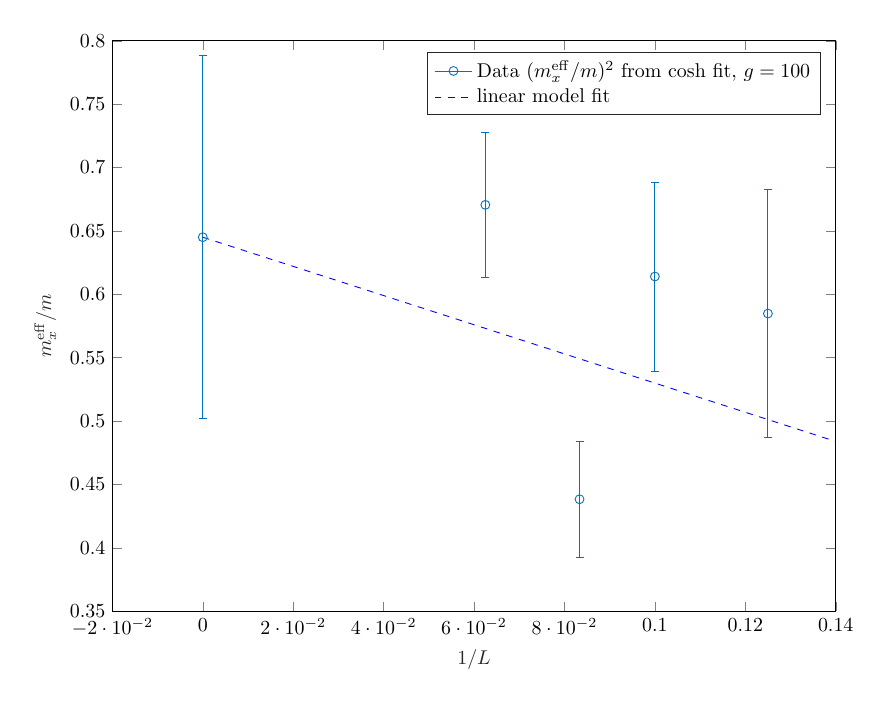
\begin{tikzpicture}[thick,scale=0.8, every node/.style={scale=0.9}]

\begin{axis}[%
width=4.521in,
height=3.566in,
at={(0.758in,0.481in)},
scale only axis,
xmin=-0.02,
xmax=0.14,
xlabel style={font=\color{white!15!black}},
xlabel={$1/L$},
ymin=0.35,
ymax=0.8,
ylabel style={font=\color{white!15!black}},
ylabel={$m_{x}^{\rm eff}/m$},
axis background/.style={fill=white},
legend style={legend cell align=left, align=left, draw=white!15!black}
]
\addplot [color=mycolor1, draw=none, mark=o, mark options={solid, mycolor1}]
 plot [error bars/.cd, y dir = both, y explicit]
 table[row sep=crcr, y error plus index=2, y error minus index=3]{%
0.0625	0.670560513952906	0.0573438887395148	0.0573438887395148\\
0.0833333333333333	0.438346924164652	0.0455068910892664	0.0455068910892664\\
0.1	0.614033856468322	0.0745890105507399	0.0745890105507399\\
0.125	0.584820357502446	0.0976223242590754	0.0976223242590754\\
0	0.645033273318665	0.143190331713913	0.143190331713913\\
};
\addlegendentry{Data $(m_x^{\rm eff}/m)^2$ from cosh fit, $g=100$}

\addplot [color=blue, dashed]
  table[row sep=crcr]{%
0	0.645033273318665\\
0.01	0.633528314410353\\
0.02	0.622023355502041\\
0.03	0.610518396593729\\
0.04	0.599013437685417\\
0.05	0.587508478777104\\
0.06	0.576003519868792\\
0.07	0.56449856096048\\
0.08	0.552993602052168\\
0.09	0.541488643143856\\
0.1	0.529983684235544\\
0.11	0.518478725327231\\
0.12	0.506973766418919\\
0.13	0.495468807510607\\
0.14	0.483963848602295\\
};
\addlegendentry{linear model fit}

\end{axis}
\end{tikzpicture}%
\caption{This plot shows a simple example of a continuum extrapolation for $m_{x\rm LAT}$ with $g=100$ in absece of a \names{Wilson} term. Every point represents a value $m_{x}^{\rm eff}(T)$ generated from one replicum with 400 field configurations each. The result of the linear regression is added as a point with errorbars at zero. \label{fig: massfit_cosh}}
\end{figure}
%
%
%
%
%
%  - - - - - - - -    cusp action   - - - - - - - - - -
%
%
%
%
\subsection{The cusp action}
To measure the action (\ref{eq: <S_cusp>}) we first explore the regime of large $g$, where we recover the following lattice observable, behaving linear in $g$ and containing a quadratic divergence in $L$ in the continuum limit
%
%
\begin{equation}
\langle S_{\rm LAT} \rangle = S_{0} + \frac{c}{2} \left(2L^{2}\right), \qquad g\gg 1.
\label{eq: S_LAT}
\end{equation}
%
%
In the continuum we would find
%
%
\begin{equation}
\langle S_{\rm cusp} \rangle = g \frac{V_{2}}{8}f'(g)  \quad \textabove{=}{$\footnotesize g\!\gg\!1$} \quad \frac{V_{2}}{2}g \equiv S_{0},
\end{equation}
%
%
leading to a possible description of $f'(g)$ given by
%
%
\begin{equation}
\frac{\langle S_{\rm cusp }\rangle}{S_{0}} = \frac{f'(g)}{4}.
\end{equation}
%
%
For a discretised version nonetheless we have to include the mass scale for the action to be dimensionless with respect to the lattice spacing
%
%
\begin{equation}
S_{0} = \frac{V_{2}}{2} m^{2}g = \frac{1}{2}\left(2L^{2}\right) M^{2} g.
\end{equation}
%
%
Furthermore we recalled the behaviour $f(g) = 4g + \text{const.} + \mathcal{O}(g^{-1})$ from (\ref{eq: scaling_fct}) and inserted $V_{2}=a^{2}(TL)=a^{2}(2L^{2})$, since we always use $T=2L$. $S_{0}$ is the discretised classical action and its value is fixed in each simulation for given $g$ and $LM$. In (\ref{eq: S_LAT}) we added a term quadratically divergent in $L$ in the continuum limit. To motivate the appearance of such behaviour let us recall that we calculate the vev of the cusp action via
%
%
\begin{equation}
 \langle S_{\rm cusp} \rangle = -g \frac{\dd \ln Z_{\rm cusp}}{\dd g}.
 \end{equation} 
 %
 %
and focus especially on any contribution to the partition function that is of quadratic order in the bosonic fermionic fields  $Z_{\rm cusp}^{(2)}=Z_{\rm B}^{(2)}Z_{\rm F}^{(2)}$. For these contributions we can schematically write
 %
 %
\begin{equation}
\begin{alignedat}{2}
Z_{\rm B}^{(2)} &= \int \prod\limits_{n=1}^{N_{\rm B}} \mathcal{D}\phi_{n} \; e^{-g \sum\limits_{i=1}^{N_{\rm B}} \int \dd t \dd s\; \phi_{i} \mathcal{O}_{i} \phi_{i}} \\
%
%
&\textabove{=}{$^{\rm LAT}$} \int \prod\limits_{n=1}^{N_{\rm B}} \left( \prod\limits_{k=1}^{\vert \mathit{\Lambda}\vert} \dd \phi_{n}^{(k)} \right) \; e^{-g \sum\limits_{i=1}^{N_{\rm B}} \phi_{i}^{\rm T}\hat{\mathcal{O}}_{i}\phi_{i}} \\
%
%
&= \prod\limits_{i=1}^{N_{\rm B}} \frac{1}{\sqrt{\det (g \hat{\mathcal{O}}_{i})}}   =    g^{-N_{\rm B}\frac{V}{2}} \prod\limits_{i=1}^{N_{\rm B}} \frac{1}{\sqrt{\det \hat{\mathcal{O}}_{i}}}  ,
\end{alignedat}
\end{equation}
%
%
where $V=\vert \mathit{\Lambda}\vert$ and $N_{\rm B}$ is the number of bosonic fields $\phi_{i}$. In the same manner we find (with the number of fermions $N_{\rm F}$)
%
%
\begin{equation}
Z_{\rm F}^{(2)}= g^{N_{\rm F}\frac{V}{2}} \pf \left(\hat{\mathcal{O}}_{\rm F} \right)
\end{equation}
%
%
and thus
%
%
\begin{equation}
\begin{alignedat}{2}
\langle S_{\rm cusp}^{(2)} \rangle &= -g \frac{\dd }{\dd g} \left( -\frac{V}{2}N_{\rm B} \ln g -\frac{1}{2} \sum\limits_{i=1}^{N_{\rm B}} \ln \left(\det \hat{\mathcal{O}}_{i}\right) + \frac{V}{2} N_{\rm F} \ln g + \ln \left( \pf \hat{\mathcal{O}}_{\rm F} \right) \right) \\
%
%
&= \frac{V}{2} \left(N_{\rm B} - N_{\rm F}\right).
\end{alignedat}
\end{equation}
%
%
This divergence with respect to the lattice volume is arising from all quadratic field contributions due to the non equality of boson and fermion numbers. After the HS transformation we have an additional amount of 17 auxiliary fields and in total 25 bosonic fields in contrast to 16 independent fermionic quantities. \\
The fermionic contribution to (\ref{eq: <S_cusp>}) is solely of quadratic order and will result in a divergent term only and is thus not relevant to measure $f'(g)$. Out of this reason it is conventional  to omit the coupling from the (pseudo) fermionic part of the action. In the observable $\langle S_{\rm LAT} \rangle$ therefore only contributes a measurement of the bosonic part of the action and thus a divergence that should be proportional to the number of bosonic fields in the large $g$ region
%
%
\begin{equation}
c\quad \textabove{=}{$\footnotesize g\!\gg\!1$} \quad N_{\rm B}.
\end{equation}
%
%
To prove this, $c$ can be determined numerically by an extrapolation with a fit linear in $1/L^{2}$ from data points for $\frac{\langle S_{\rm LAT}\rangle}{2L^{2}} = \frac{c}{2}+ \frac{S_{0}}{2L^{2}}$.